\chapter{Dataset Generation \& Annotation}
\label{section:Dataset}

\section{Introduction}
\section{Analysis}
Generating a Mean Payoff Game can be decomposed into two subsequent objectives.
\begin{enumerate}
	\item Generate the Graph itself.
	\item Generate the Weights
\end{enumerate}


\section{Graph Distributions}
There are many well studied graph distributions in the litterature. One of the most explored ones are the $\mathcal{G}(n,p)$ and $\mathcal{G}(n,m)$ families.

We will offer here a directed variant of these two distributions that suits for \acrshortpl{mpg}.
\subsection{$\Dnp{n}{p}$ Family}
For $n\in\mathbb{N},p\in[0,1],$ a di-graph $G=(\VertexSet,\EdgeSet)$ is said to follow a $\Dnp{n}{p}$ distribution if $\lvert \VertexSet \rvert=n$ and:
$$
\forall e\in \VertexSet\times \VertexSet, \quad \mathscr{P}(s\in \EdgeSet)=p
$$
This is the directed version of the binomial random graph distribution $\mathcal{G}(n,p)$ \cite[Section.~1.1]{RandomGraphs}.

\subsection{$\Dnm{n}{m}$ Family}
For $n\in\mathbb{N},m\in\mathbb{N},$ a graph $G$ is said to follow a $\mathcal{G}(n,m)$ distribution if $\lvert V \rvert=n,\lvert  E \rvert=m$ and the edges $e_1,\dots,e_m$ were drawn uniformly and without replacement from the set $\VertexSet\times \VertexSet$

This is the directed version of the uniform random graph distribution $\mathcal{G}(n,m)$ \cite[Section.~1.1]{RandomGraphs}.

While $\Dnm{n}{m}$ has a more natural definition, the analysis of $\Dnp{n}{p}$ is easier. Also there are many results showing similarities between the two distributions \cite[Section.~1.1]{RandomGraphs}. For this reason, we will focus primarily on $\Dnm{n}{p}$ graphs.

\subsection{$\Dnp{n}{p}$ Graph Construction}

\subsubsection{Naive Method}
The definition of $\mathcal{D}(n,p)$ gives a straightforward construction. \newline
This is achieved by flipping a coin\footnote{The coin is potentially biased with a probability of obtaining head equal to $p\in [0,1]$} for each pair of node $(u,v)\in V^2$, we add an edge if we get a Head. 
\newline This is implemented in the following algorithm:
\begin{algorithm}
	\caption{$\mathcal{D}(n,p)$ Graph Generation}\label{alg:Dnp_Naive}
	\begin{algorithmic}
		\Require $n\in\mathbb{N}^*$ the size of the graph
		\Require $p\in\mathbb{N}^*$ the edge probability 
		\Ensure $G\sim \mathcal{D}(n,p)$  
		\State $A:(u,v)\in V\times V\rightarrow 0$
		\For{ $u\in V$} 
		\For { $v \in V$ }
		\State Generate $X\sim \mathcal{B}(p)$
		\Comment{$\mathcal{B}(p)$ is the bernoulli distribution}
		\State $A(u,v)\leftarrow X$
		\EndFor
		\EndFor
		\State \Return $G\leftarrow \texttt{GraphFromAdjacencyMatrix}(A)$
	\end{algorithmic}
\end{algorithm}
\FloatBarrier
The complexity\footnote{We assume the cost of generating a Bernoulli random variable as $\mathcal{O}(1)$} of the following algorithm is $\mathcal{O}(n^2).$
\subsubsection{Optimized Method}
Instead of iterating over all possible pair of nodes. For each vertex $v\in V$:
\begin{itemize}
	\item We can sample a number $d$ from the outgoing degree distribution\footnote{Or the ingoing degree distribution, they are in fact equal.}
	\item We then choose $d$ numbers uniformly without replacement from an indexable representation of $V$
\end{itemize}
The following algorithm implements the optimized method:
\begin{algorithm}
	\caption{$\mathcal{D}(n,p)$ Graph Generation Optimisation}\label{alg:Dnp_Fast}
	\begin{algorithmic}
		\Require $n\in\mathbb{N}^*$ the size of the graph
		\Require $p\in\mathbb{N}^*$ the edge probability 
		\Ensure $G\sim \mathcal{D}(n,p)$  
		\State $A:u\in V\rightarrow \varnothing$
		\For{ $u\in V$} 
		\State Generate $d\sim \mathcal{B}(n,p)$
		\Comment{$d$ represents the degree, $\mathcal{B}(n,p)$ is the binomial distribution}
		\State $A(u)\leftarrow \choice(V,d)$
		\EndFor
		\State \Return $G\leftarrow \texttt{GraphFromAdjacencyList}(A)$
	\end{algorithmic}
\end{algorithm}
\FloatBarrier
Now, let $C(a,b)$ be the cost of choice function. 
\newline The expected complexity of this algorithm as a function of $n=\lvert \VertexSet \rvert$ and the degrees $d_1,\dots,d_n$ is:
\begin{align}
	\label{eqn:DnpBigO}
	\tilde{\mathcal{O}}\left(\sum_{i=1}^n1+\mathbb{E}[C(n,d_i)]\right) &= 	\tilde{\mathcal{O}}\left(n+\sum_{i=1}^n\mathbb{E}[C(n,d_i)]\right) 
\end{align}
We will show on the next section what choice function should we use.
\subsection{Choice Function}
\subsubsection{First Proposition}
We propose here a simple choice algorithm, but it is still efficient for our use case.
\newline It works simply by drawing without replacement, but we ignore duplicate elements. This is implemented as follow
\begin{algorithm}
	\caption{$\mathcal{D}(n,p)$ Choice without replacement}\label{alg:Choice}
	\begin{algorithmic}
		\Require $S$ a list
		\Require $m\in\{0,\dots \lvert S \rvert\}$ the number of chosen elements
		\Ensure $H$ a set of size $m$ containing uniformly drawn elements without replacement. 
		\State $H\leftarrow \varnothing$
		\While{$\lvert H \rvert < m$}
			\State Generate $v\sim \mathcal{U}(S)$ 
			\Comment{Where $\mathcal{U}(S)$ is the uniform distribution over $S$}
			\State $H\leftarrow H \cup \{v\}$
		\EndWhile
		\State \Return $H$
	\end{algorithmic}
\end{algorithm}
\FloatBarrier
To estimate the cost of this algorithm, we will use probabilistic reasoning.
\newline Let $X_{n,m}=C(n,m)$ the running time of an execution of algorithm \ref{alg:Choice} in a set $S$ of size $n$, with $m$ elements to be chosen.
We have:
\begin{align*}
	X_{n,0} & \ \text{is deterministic}\\
	X_{n,0}&=\mathcal{O}(1) \\
	\mathbb{E}[X_{n,m}]&=1+\frac{1}{n}\sum_{k=0}^{n-1} \mathbb{E}[X_{n,m} \mid \text{The last drawn number is}\ k] \\
	&=1+\frac{1}{n}\sum_{k=0}^{m-2} \mathbb{E}[X_{n,m}]+\frac{1}{n}\sum_{k=m-1}^{n-1} \mathbb{E}[X_{n,m-1}] \\
	&= 1+\frac{m-1}{n}\mathbb{E}[X_{n,m}]+\frac{n-m+1}{n}\mathbb{E}[X_{n,m-1}]
\end{align*}
Now we arrived at a recurrent formula. We will simplify it as shown below:
\begin{align*}
\frac{n-m+1}{n}\mathbb{E}[X_{n,m}]&=\frac{n-m+1}{n}\mathbb{E}[X_{n,m-1}] +1\\
\implies \mathbb{E}[X_{n,m}]&=\frac{n-m+1}{n-m+1}\mathbb{E}[X_{n,m-1}]+\frac{n}{n-m+1}\\
&=\mathbb{E}[X_{n,m-1}]+\frac{n}{n-m+1} \\
&=\sum_{k=1}^m\frac{n}{n-k+1}+\mathcal{O}(1)\\
&=\sum_{k=0}^{m-1}\frac{n}{n-k}+\mathcal{O}(1) \\
&=n\sum_{k=n-m+1}^n\frac{1}{k}+\mathcal{O}(1)\\
&=n(H_n-H_{n-m})+\mathcal{O}(1)
\end{align*}
Here $(H)_{n\in\mathbb{N}^*}$ is the harmonic series, and we define $H_0=0.$
\subsubsection{Complexity}
%Prooof!!!
The expected complexity of algorithm \ref{alg:Choice} depends on both $n$ and $m$:
\begin{itemize}
	\item If $m=kn+o(n)$ with $k\in\mathopen]0,1\mathclose[$, then it is $\tilde{\mathcal{O}}(m).$
	\item If $m=n-o(n)$, It is\footnote{Here we use the minus sign to emphasize that $m\le n$} $\tilde{\mathcal{O}}(m\log m).$ 
\end{itemize}
To prove this result, we use a well-known asymptotic approximation of the Harmonic series\footnote{This asymptotic approximation can be proven using the Euler–Maclaurin formula} \cite[Section~1.2.11.2]{ArtComputerProgramming}:
$$
H_n=\ln n+\gamma -\frac{1}{2n}+\mathcal{O}\left(\frac{1}{n^2}\right)
$$
We can prove this claim as follow for $m=km+o(m),k\in \mathopen[0,1\mathclose[$:
\begin{align}
	\mathbb{E}[C(n,m)]&=-n\ln \left(1-\frac{m}{n}\right) -\frac{1}{2}\left(1-\frac{n}{n-m}\right)+\mathcal{O}\left(\frac{1}{n}\right) \nonumber \\
&=-n\ln (1-k+o(1))+\frac{1}{n}(1-\tfrac{1}{1-k+o(1)})+\mathcal{O}(\tfrac{1}{n}) \label{eqn:ChoiceBigO} \\
&=\mathcal{O}(m) \nonumber
\end{align}
For $m=n-o(n),$ we prove it by noting that:
\begin{align*}
\mathbb{E}[C(n,m)]&\le\mathbb{E}[C(n,n)]= \mathcal{O} (nH_n) =\mathcal{O}(m\log m)
\end{align*}
\newpage
\subsubsection{Refinement}
If $m$ tends to $n,$ it is more hard to select $m$ elements from a set of size $n$ without replacement. This explains the extra logarithmic factor.
\newline In that case, we can instead focus on the dual problem: ``Find the $n-m$ elements that will not be selected". This can be calculated in $\mathcal{O}(n-m).$
\newline Once we find the elements that will not be selected, their set complement are exactly the $m$ elements that will be selected. This new algorithm is guaranteed to be $\mathcal{O}(m)$ irrespective of $n$ and $m$
\begin{algorithm}
	\caption{Fine tuned $\mathcal{D}(n,p)$ Choice without replacement }\label{alg:ChoiceFineTuned}
	\begin{algorithmic}
		\Require $S$ a list
		\Require $m\in\{0,\dots \lvert S \rvert\}$ the number of chosen elements
		\Require $\choice$ The choice function defined on algorithm \ref{alg:Choice}
		\Require $\tau$ a fine tuned threshold. We will use $\tau=\frac{1}{2}$ for all practical purposes.
		\Ensure $H$ a set of size $m$ containing uniformly drawn elements without replacement. 
		\If {$\frac{m}{\lvert S \rvert} \le \tau$}
			\State $H\leftarrow \choice(V,n)$
		\Else
			\State $H\leftarrow S\setminus \choice(S,n-m)$
		\EndIf
		\State \Return $H$
	\end{algorithmic}
\end{algorithm}
\FloatBarrier
Also, an important point is that by combining the analysis of all possible cases, we can extract a constant factor that is independent\footnote{The independence can be proven by taking the supremum of the right-hand side of equation \eqref{eqn:ChoiceBigO} over $[0,\tau]$, and the fact that $\tau$ is fixed.} of $n.$ So that the Big-O bound is only a dependent on $m$.
\subsection{Complexity of Optimised $\mathcal{D}(n,p)$ Graph Construction}
Now, using algorithm \ref{alg:ChoiceFineTuned} as the choice algorithm, we can further simplify equation \eqref{eqn:DnpBigO} as a function of only $n=\lvert \VertexSet\rvert$ and $m=\lvert \EdgeSet\rvert.$
\newline This proves that $\Dnp{n}{p}$ construction can be achieved in expected linear time:
\begin{align*}
	\tilde{\mathcal{O}}\left(n+\sum_{i=1}^n\mathbb{E}[C(n,d_i)]\right)  &= \tilde{\mathcal{O}}\left(n+\sum_{i=1}^nd_i\right) \\
	&=\tilde{\mathcal{O}}\left(n+m\right)
\end{align*}

\begin{figure}[H]
	\centering
	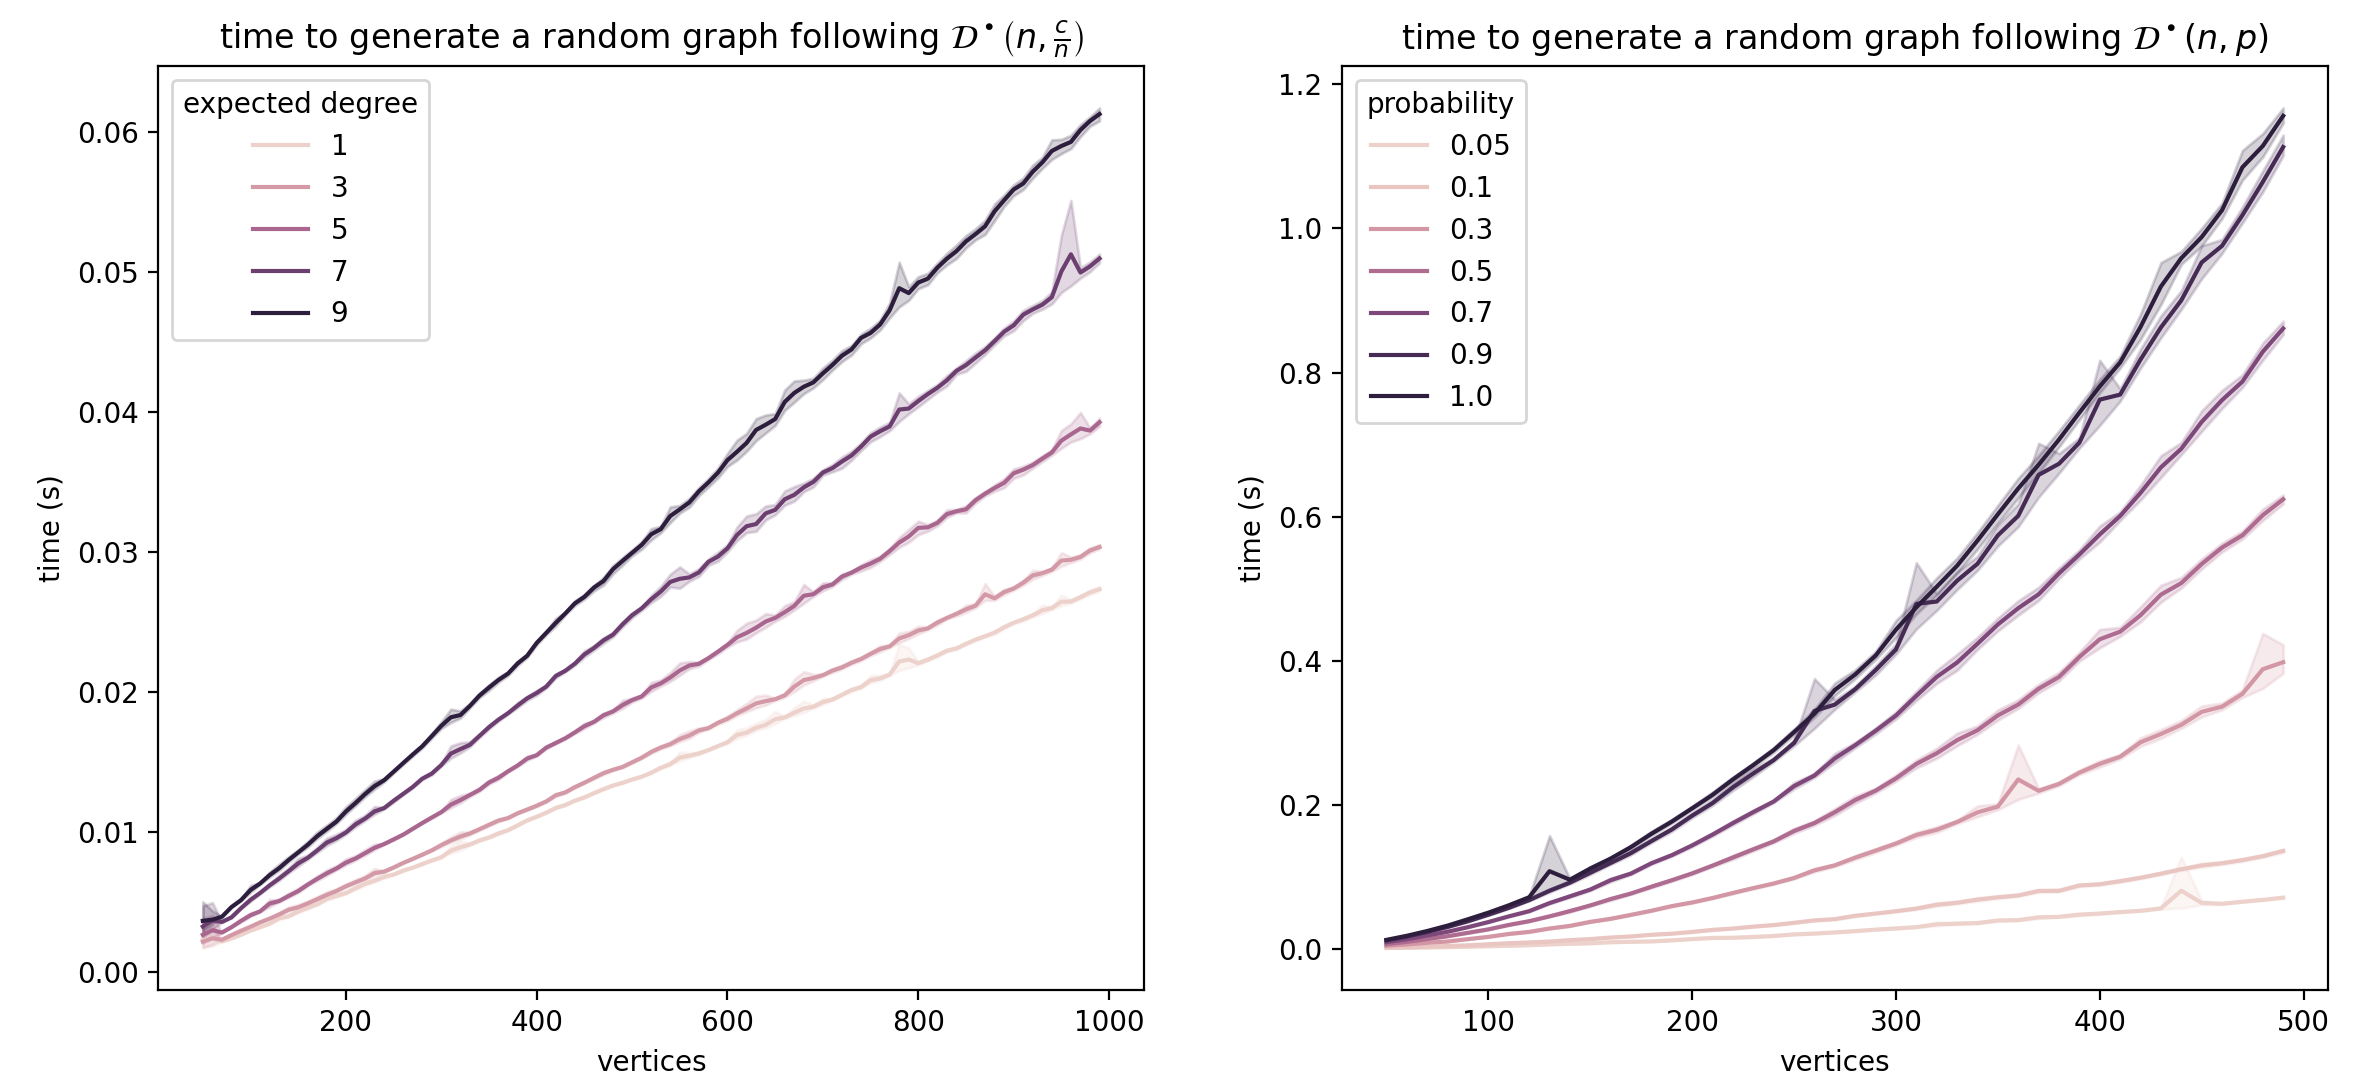
\includegraphics[width=0.95\textwidth]{Figures/GraphGen.png}
	\caption{Experimental performance to generate dense \& sparse graphs}
\end{figure}
\FloatBarrier

\subsection{$\mathcal{D}(n,m)$ Construction}
To construct a random $\mathcal{D}(n,m)$ graph, we only have to select $m$ uniformly random elements from the set $V\times V.$
\newline We will use algorithm \ref{alg:ChoiceFineTuned} for this purpose\footnote{It is essential that the list $V\times V$ be lazy loaded. In particular, each element will only be loaded when it is indexed. This is essential to reduce the complexity. Otherwise, we will be stuck in an $\mathcal{O}(n^2)$ algorithm.}:
\begin{algorithm}
	\caption{Fine tuned $\mathcal{D}(n,p)$ Choice without replacement }\label{Dnm} 
	\begin{algorithmic}
		\Require $n\in\mathbb{N}^*$
		\Require $m\in\{0,\dots,n^2\}$ the number of chosen elements
		\Ensure $G\sim \mathcal{D}(n,m)$
		\State $E\leftarrow \choice(\text{Lazy}(V)\times \text{Lazy}(V),m)$ \Comment{We only need the $m$ elements on-demand.}
		\State \Return $G\leftarrow \text{GraphFromEdges}(E)$\Comment{This justifies using \text{Lazy}}
	\end{algorithmic}
\end{algorithm}
\FloatBarrier
Here $\text{Lazy}(V)\times \text{Lazy}(V)$ is a lazy implementation of cartesian product that supports bijective indexing\footnote{Indexing is required for uniform sampling} over $\{0,\dots,n^2-1\}.$
\newline The complexity of this construction is: $
\tilde{\mathcal{O}}(m)
$ 

\section{Sinkless Conditionning}
Sampling from a graph distribution may lead to graphs that have at least one sink. 
\newline These graphs are problematic as Mean Payoff Graphs are exactly the sinkless graphs.
\newline To migitate this, we will impose a conditionning on both distribution that will gives a guaranteed Mean Payoff Graph.
\newline We will explore such conditionning both distribution:
\begin{itemize}
	\item $\mathcal{D}^\bullet(n,p):$ This is the distribution of graphs following $\Dnp{n}{p}$ with the requirement that they do not have a sink.
	\item $\mathcal{D}^\bullet(n,m):$ This is the distribution of graphs following $\Dnm{n}{m}$ with the requirement that they do not have a sink.
\end{itemize}
\subsection{Graph Rejection Construction}
\subsubsection{Estimating Complexity}
Now the method of rejecting graphs that have sinks and retrying give us a natural question about how many times will the algorithm reject graph until finding a desirable one.\newline
The number of such rejections will follow a geometric law $\mathcal{G}(h(n,p))$ where: 
\begin{equation}
	\label{eqn:HnpProbability}
	h(n,p)=\mathscr{P}\left(\text{Sinkless}(\mathcal{D}(n,p))\right)=(1-(1-p)^n)^n
\end{equation}
Proof of \eqref{eqn:HnpProbability} is found in section \ref{section:RandomGraphs:PropertyProbability}
\newline With that, the expected complexity of the algorithm will be:
$$
\tilde{\mathcal{O}}\left(\frac{C(n,p)}{h(n,p)}\right)=\tilde{\mathcal{O}}\left(\frac{C(n,p)}{(1-(1-p)^n)^n}\right)
$$
With $C(n,p)$ the cost of building the graph, depending on the algorithm\footnote{The two algorithms that we have discussed are the naive $\mathcal{O}(n^2)$ algorithm and the more optimized $\tilde{\mathcal{O}}(n+m)$ algorithm.}.
\paragraph{Dense Graph case}
Now it is clear for dense enough graphs, in particular with $p(n) \ge \frac{\ln (n)}{n}$ for large enough $n$, the expected complexity will reduce to $\mathcal{O}(C(n,p))$. This is a result of equation \eqref{eqn:SinklessProbabilityLimit}.
\newline In the dense case, we consider the rejection method to be efficient.
\paragraph{Sparse Graph case}
If $p(n)=\frac{k\ln n}{n}+c$ with $k<1.$ We have as a result of:
$$
(1-(1-p)^n)^n=e^{-e^{-c}x^{1-k}+o(x^{1-k})}
$$
With that, the expected complexity of the rejection method will be:
$$
\tilde{\mathcal{O}}\left(C(n,p)\times \exp\left(e^{-c}x^{1-k}+o(x^{1-k})\right)\right)
$$
which is an exponential algorithm, and thus inefficient for large graphs.
Since property $\mathtt{P}$ is increasing, this argument generalises to $p(n) \le \frac{k\ln n}{n}+c$ for large enough $n$
\begin{figure}[H]
	\centering
	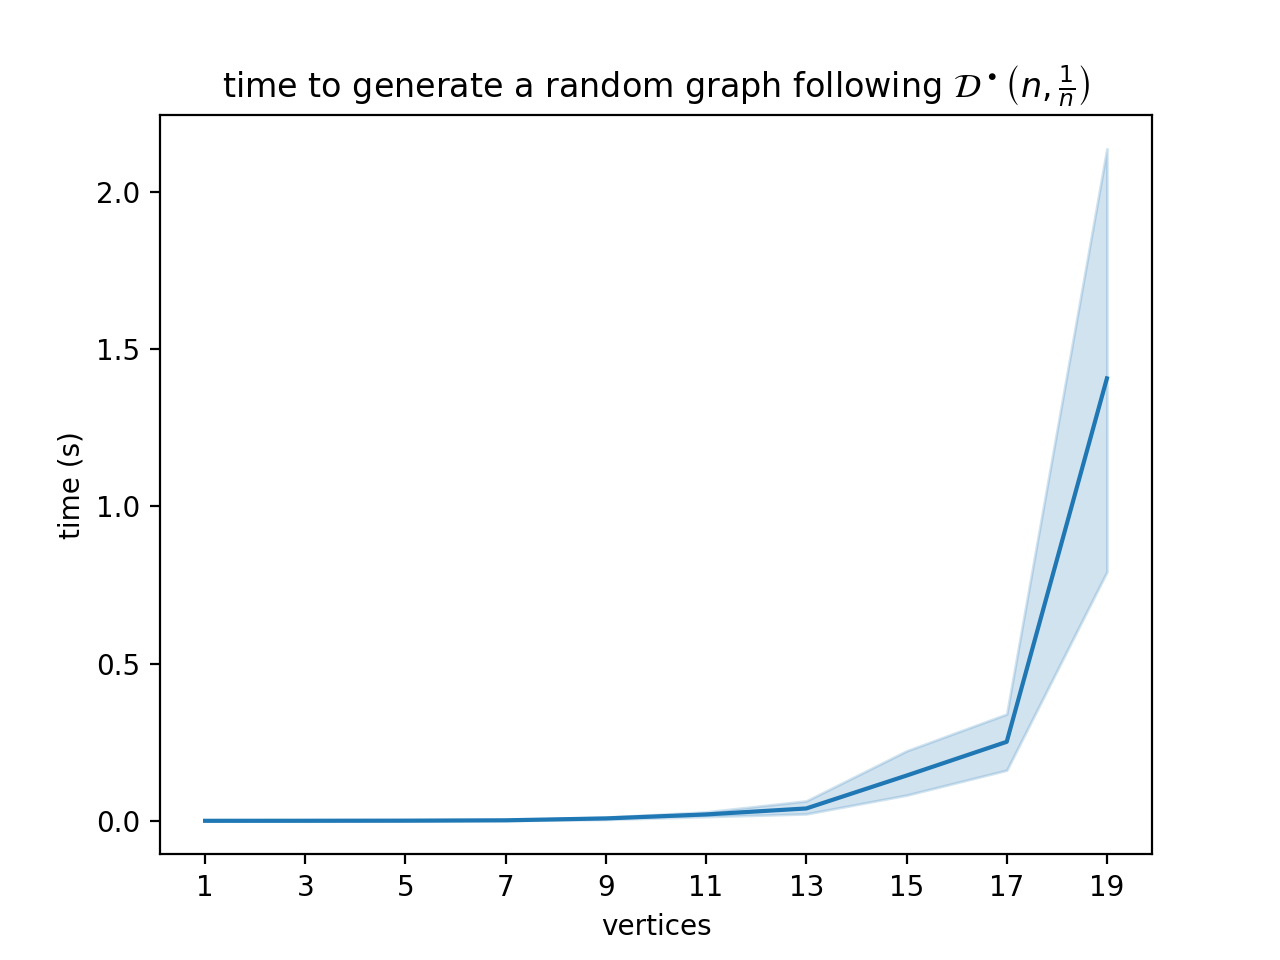
\includegraphics[width=0.75\textwidth]{Figures/BadSparseGraphGen.png}
	\caption{Exponential blowup when using the graph rejection method}
\end{figure}
\FloatBarrier
\subsection{Degree Rejection Construction}
\label{section:Dataset:Sinkless:DegreeRejection}
Instead of throwing the whole graph at once. For every vertex $u\in V,$ we try to construct the adjacenty vertices of $u,$ and repeat if the procedure gives $\Adj u =\varnothing$
\newline With this trick, the expected complexity will reduce for both algorithms to:
$$
\tilde{\mathcal{O}}\left(\frac{C(n,p)}{1-(1-p)^n}\right)
$$
Now for our case, it is natural to assume that $p(n) \ge \frac{1}{n},$ as a Mean Payoff Graph does not have a sink. With that: 
$$
1-(1-p)^n \ge 1-(1-\tfrac{1}{n})^n \ge 1-e^{-1}
$$
Therefore, the expected complexity will simplify to:
$$
\tilde{\mathcal{O}}\left(C(n,p)\right)
$$
Moreover, the cost of the conditionning makes at most a constant $\frac{1}{1-e^{-1}}\approx 1.582$ factor slowdown, which is effectively neligible.

\begin{figure}[H]
	\centering
	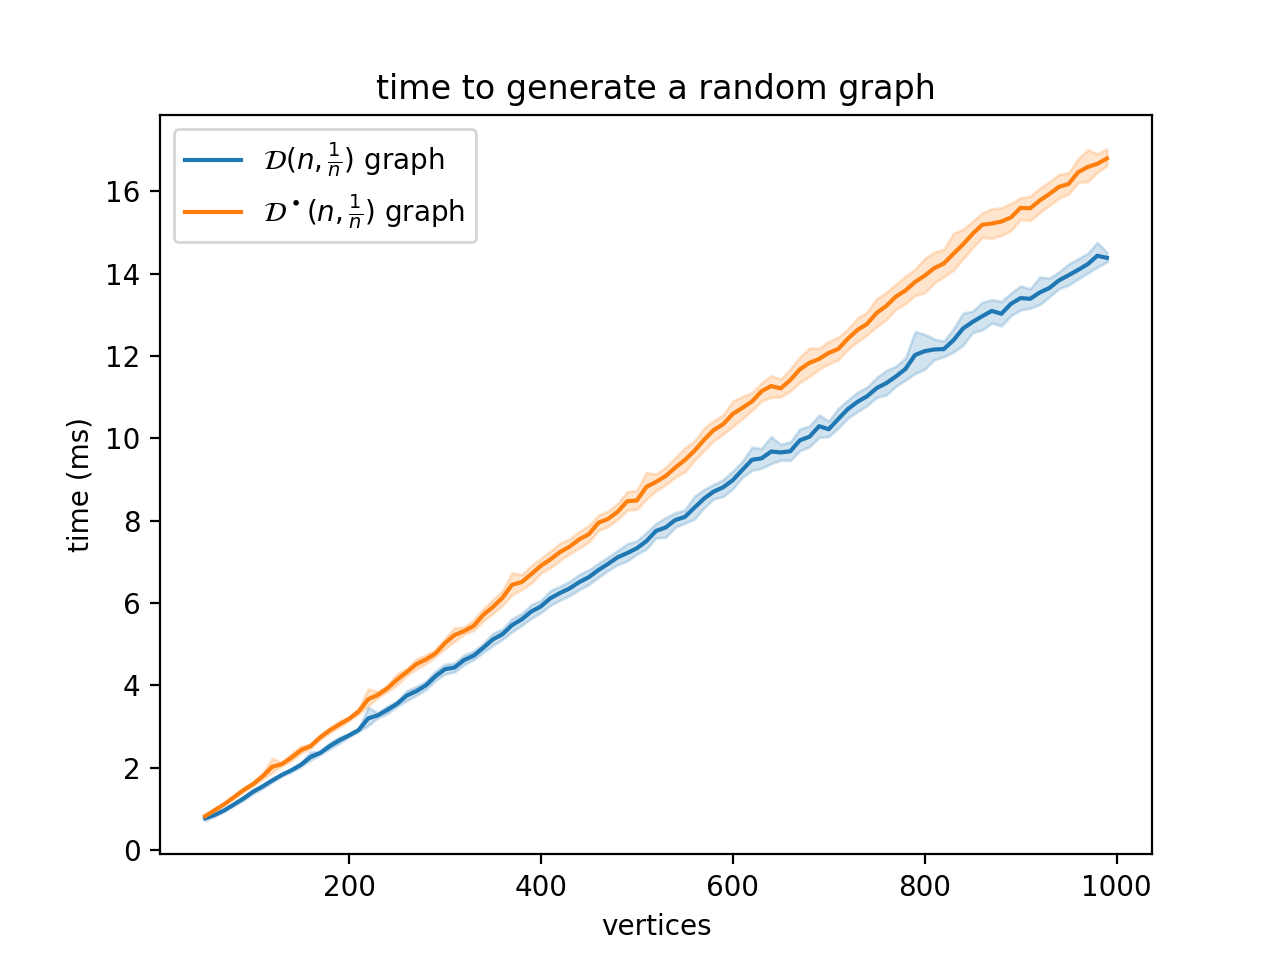
\includegraphics[width=0.75\textwidth]{Figures/DegreeSparseGraphGen.png}
	\caption{Small slowdown due to the degree rejection method}
\end{figure}
\FloatBarrier

%\section{Weights Distribution}
%\subsection{Construction}
%Once the graph is constructed. We only have to %generate the weights. \newline
%This will be done by creating a random weight %function:
%$$
%W(u,v):(u,v)\rightarrow W_{u,v}
%$$
%Here $W_{u,v}$ will be a sequence of real %random variables. \newline
%In our case, we set $(W_{u,v})_{(u,v)\in E}$ to %be independent and identically distributed over %a real distribution $\mathcal{W}.$ 

\section{Proposed \acrshort{mpg} distributions}
\subsection{Desired properties of \acrshort{mpg} distributions}
\subsubsection{Fairness}
This is essential, as we intend to generate a sequence of Mean Payoff Games that do not favour statistically a certain player.

A game distribution is said to be fair if:
\begin{equation}
	\label{eqn:Fairness}
	\mathscr{P}(\Max \text{wins}\ G \ \text{assuming optimal strategies} ) = 	\mathscr{P}(\Min \text{wins}\ G \ \text{assuming optimal strategies} )
\end{equation}
Furthermore, if we assume $C_2$ or $C_3$ as the winning conditions, \eqref{eqn:Fairness} is equivalent to the following equation:
\begin{equation*}
	\mathscr{P}(v(G) > 0) = \mathscr{P}(v(G) < 0)
\end{equation*}
\subsubsection{Symmetric}
A real distribution is said to be symmetric if:
$$
\forall [a,b]\in \mathbb{R},X\sim \mathcal{W},\quad \mathscr{P}(X\in [a,b]) = \mathscr{P}(X\in [-b,-a])
$$
We will define a symmetric Mean Payoff Game distribution as a distribution of Mean Payoff Game whose weights are independent and identically distributed on a symmetric real distribution.

We will require a symmetric \acrshort{mpg} as we do not want a player to have an inherit advantage over the other one\footnote{Other than the first move.}
\subsection{Implemented Distributions}
The following table resumes the implemented distributions:
\begin{table}[h]
	\small
	\begin{tabularx}{\textwidth}{| X | X | X |}
		\hline
		
		Distribution Family & Parameters & Type  \\
		\hline
		$\mathcal{D}(n,p)$ & \vspace{-5mm}
		\begin{itemize}
			  \setlength\itemsep{0em}
			\item $n:$ Graph size
			\item $p:$ Edge probability
		\end{itemize} & Graph distribution \\
		\hline
		$\mathcal{D}(n,m)$ & 
		\vspace{-5mm}
		\begin{itemize}
			  \setlength\itemsep{0em}
			\item $n:$ Graph size
			\item $m:$ Number of edges
		\end{itemize} & Graph distrbiution  \\
		\hline
		$\mathcal{U}_{\text{discrete}}(-r,r)$ &
		\vspace{-5mm}
		\begin{itemize}
			  \setlength\itemsep{0em}
			\item $r:$ The radius of the support
		\end{itemize}
		 &  Weight distribution\\
		\hline
		$\mathcal{U}(-r,r)$ &\vspace{-5mm}
		\begin{itemize}
			  \setlength\itemsep{0em}
			\item $r:$ The radius of the support
		\end{itemize} & Weight distribution \\
		\hline
		$\mathcal{N}(0,\sigma)$ &
		\vspace{-5mm}
		\begin{itemize}
			  \setlength\itemsep{0em}
			\item $\sigma:$ The standard deviation
		\end{itemize} & Weight distribution\\ 
		\hline 
		
	\end{tabularx}
	\caption{Le tableau d'avancement des BNNs
	\label{table:Distributions}}
\end{table}
\FloatBarrier
Also, to generate the initial state, we have defaulted to:
\begin{itemize}
	\item The uniform distribution over the vertices to generate the starting vertex
	\item The bernoulli distribution to generate the starting player.
\end{itemize}
With all that said, distributions are fair in the limit and are symmetric, provided that the underlying graph distribution and weight distribution are chosen from the table \ref{table:Distributions}.

\section{MPG Generation}
\label{section:MPG:Generation}
\subsection{Distribution}
\label{section:MPG:Generation:Distribution}
\begin{itemize}
	\item Each generated graph will follow a distribution $\mathcal{G}(n,p(n))$  for some $n\in\mathbb{N}^*$
	\item The weights will follow the discrete uniform distribution $\mathcal{D}(-1000,1000)$

\end{itemize}

We will generate two kinds of datasets, depending on the nature of the graph

\subsubsection{Dense Graphs}
\begin{itemize}
	\item Let $\mathcal{P}=\{0.1,0.2,0.3,0.5,0.7,0.8,0.9,1\}$
	\item $\mathcal{N}=\{10,20,30,40,50,60,70,80,90,100,110,120,130,140,150,200,250,300,400,500\}$
	\item For each $(n,p)\in \mathcal{N}\times \mathcal{P},$ we will generate $K=1000$ observations $G^{n,p}_1,\dots,G^{n,p}_{K} \sim \mathcal{G}(n,p)$ 
\end{itemize} 

The total number of examples is:
$$
K\times\lvert \mathcal{N} \rvert \times \lvert \mathcal{P}\rvert=160000
$$
\subsubsection{Sparse Graphs}
\subsection{Implementation}
We have implemented a python application called 
\subsection{Deployment}
We have deployed the pipeline in the HPC system. We have launched the following command.
\newline The figure below shows the pipeline:
\begin{figure}[H]
	\centering
	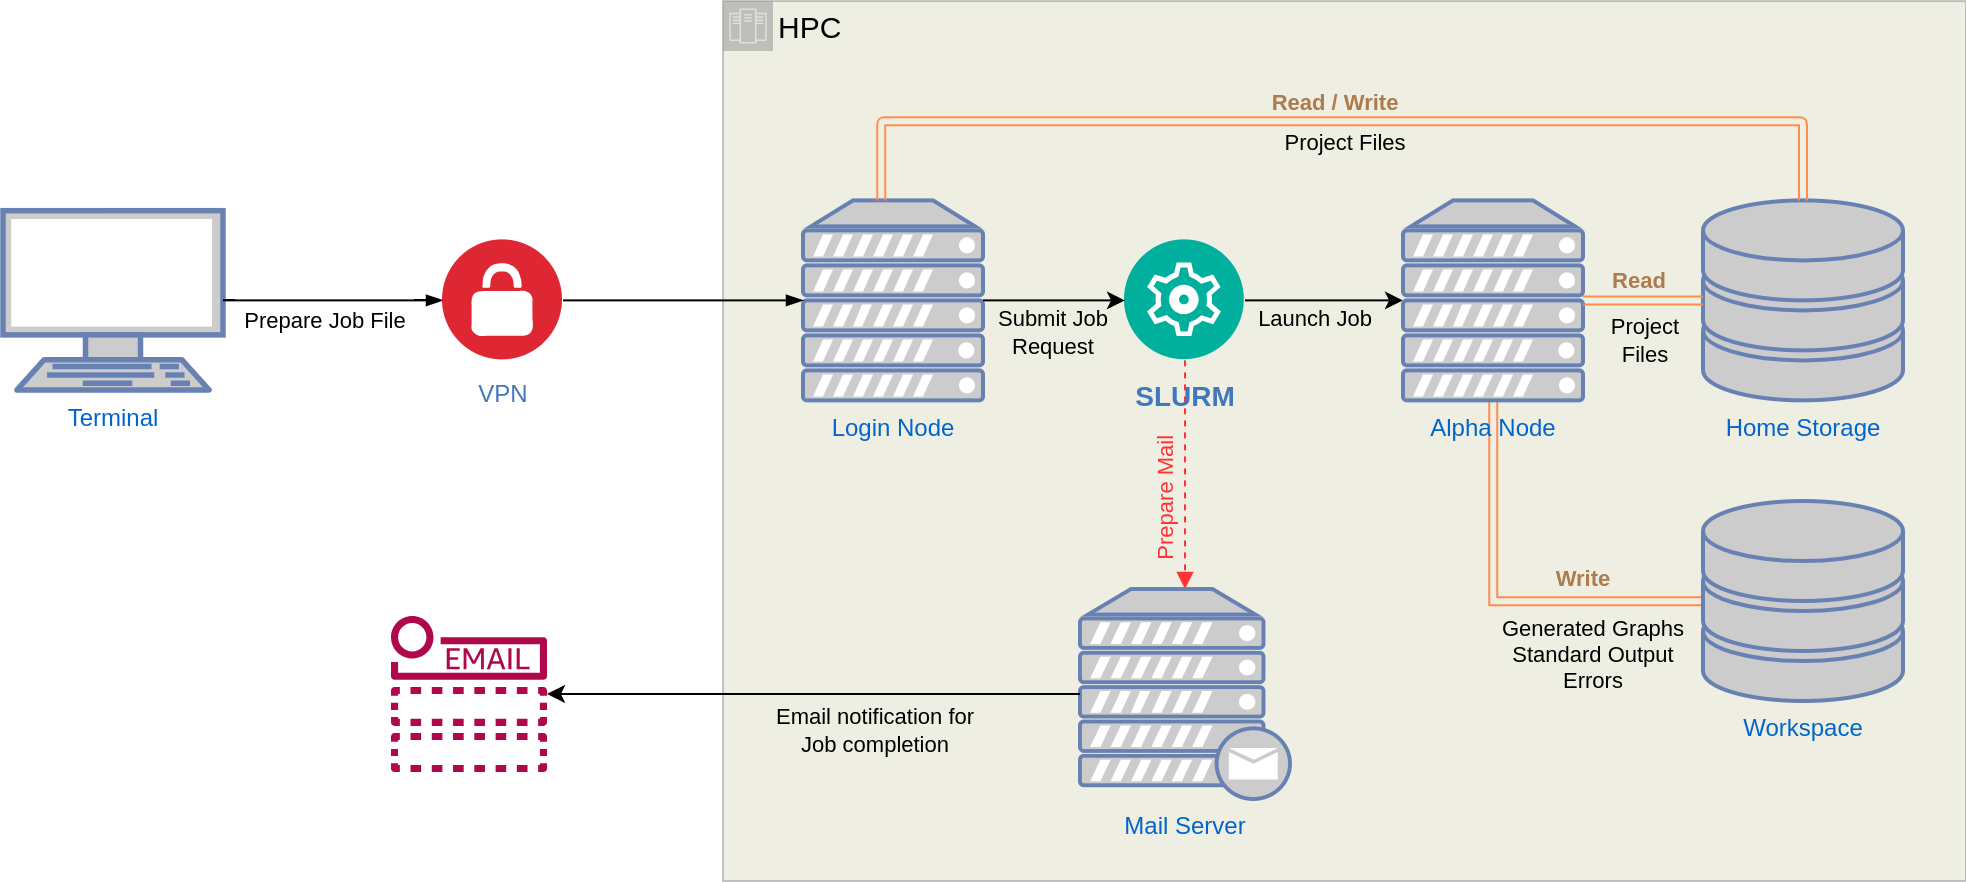
\includegraphics[width=0.95\textwidth]{Figures/DatasetGeneration.png}
	\caption{HPC pipeline to generate mean payoff graphs}
\end{figure}
\FloatBarrier
The generation was done on a `haswell64` partition with 24 cores. and it took 02:12:38 hours.

\section{Annotation}
\subsection{Approach}
We used the \acrfull{csp} algorithm $\ref{alg:AC3Optimized}$ to annotate the dataset, potentially augmented with some heuristics.

We implemented a program that takes the path of the dataset, and solves the Mean Payoff Games one by one.

To maximize efficiency, the program launches many solver threads, with each one independently working on a single file, and the results are accumulated using a ConcurrentQueue.
\subsection{Target Values}
The solver will calculate the following targets:
\begin{itemize}
	\item The optimal pair of strategies
	\item The mean payoffs for each starting position, turn.
	\item The winners for each starting position, turn.
\end{itemize}
Also, some additional metadata are generated for analysis:
\begin{itemize}
	\item \texttt{dataset}: The name of the whole dataset
	\item \texttt{graph}: The name of the graph.
	\item \texttt{status}: The solver's status on the given graph. In particular, whether it succeeded to solve the instance or not\footnote{We expect that the solver may crash due to several reasons (corrupted file, out of memory, etc\dots). For that we made additional effort for exception handling, so that an error for a single instance does not propagate to the whole program.}. Equal to ``OK" if the execution is successful.
	\item \texttt{running\_time}: The time needed to solve the instance.

\end{itemize}

\subsection{Heuristics}
To accelerate the annotation of the two datasets, we had to apply some heuristics to the algorithm. We made essentially two kinds of heuristics.
\subsubsection{Linear Bound}
This is the heuristic based on the view that for almost all solutions of a Ternary Max Atom system extracted from our generated random games, either:
\begin{itemize}
	\item All variables are infinite: 
	$$
	X(u)=-\infty \quad \forall u\in V$$
	\item The diameter of assignments is in the order of $\lVert W\rVert_{\infty}$
	$$
	\Delta X = \sup_{u\in V}X(u)-\inf_{u\in V,X(u)>-\infty}X(u)= \mathcal{O}(\lVert W\rVert_{\infty})$$
\end{itemize}
This heuristic suggests a much tighter search space to the worst case $\lVert W \rVert_{1}$ one. 
\newline
We believe this heuristic arises due to the random property of graphs, because in general, one can build an infinite family of ternary max atom systems that violate this heuristic. \newline In fact, going further, one can build a family of ternary max atom systems were the $\lVert W \rVert_{1}$ estimation is tight. This is demonstrated in the following figure:
\begin{figure}[H]
	\begin{align*}
		\begin{cases}
			X_0 &\le \max(X_{0},X_{1}) -1 \\
			\dots  & \dots \\
			X_{n-1} & \le \max(X_{n-1},X_{n})-1
		\end{cases}
	\end{align*}
	\caption{A counter example to the Linear Bound heuristic}
\end{figure}
\FloatBarrier
To generate the dataset, we applied this heuristic with $\Delta X=4\lVert W\rVert_{\infty}$
$$
D = \{-\infty,-2 \lVert W\rVert_{\infty},,-2 \lVert W\rVert_{\infty}+1 ,\dots ,2\lVert W\rVert_{\infty} \}
$$

\subsubsection{Early Stopping}
If after any iteration of arc consistency, $\max_{x\in V}\nu(x) < \sup D.$ Then, $\nu(t)$ will converge to $-\infty$ for all $t.$ 
\newline Thus, we stop the algorithm and sets $\nu(t)\leftarrow -\infty,\quad \forall t$
\begin{proof} 
suppose that in fact there is an assignment with: 
$$
-\infty < \max_{u\in V}\nu(u) < \sup D$$
We will take the $u$ with the biggest such $\nu(u).$  
\newline Now our system is a tropical max atom system, which means translations are also a polymorphism of this system, so for any assignment $\nu:V\rightarrow\mathbb{Z},\ X+t$ is also an assignment $\forall t\in \mathbb{Z}.$ With that, $\nu+\sup D-\nu(u)$ is also an assignment.
\newline This assignment has the property: $$
\forall s\in V,\quad \nu(s)+\sup D-\nu(u) \in D
$$
Which is a contradiction, as it violates the consistency of arc consistency, and the maximality of the solution with respect to the domain $D$
\end{proof}
  
The efficiency of the Early Stopping heuristic depends on the density of the graph. Empirically, for dense graphs. the analoguous ternary max atom system usually has two kind of assignments:
\begin{enumerate}
	\item Either all variables are finite
	\item Either all variables are $-\infty$
\end{enumerate}
This translates back in a dense Mean Payoff setting, that the winner of the game usually does not depend in the starting position and the starting turn. 
\newline With that, the Early Stopping heuristic will quickly detect the second case, which we believe as the hurdle of the algorithm.
\newline On the other hand, for sparse graphs, we do not have this nice distinction between finite and infinite assignments, and they can overlap, and so will make this heuristic useless in practice.

\subsection{Implementation}
\subsubsection{Algorithm}
We implemented a Mean Payoff Graph solver. It calculates the optimal move for each player in each position. Thus, our implementation gives an exact solution to the optimization problem\footnote{In its current version, It gives a weak optimal strategy for both players $\Max,$ and $\Min.$ The winning condition is $C_2$ }  for Mean Payoff Games.
\newline It works by a transforming a mean payoff game to an equivalent min-max system, then applying two subsequent reductions to a $n$-ary max atom system, then to a ternary max atom system. The solution of the latter is propagated back to mean payoff game to induce an optimal strategy.
\begin{algorithm}
	\caption{Solving a Mean Payoff Graph for all states}\label{alg:MPGSolver}
	\begin{algorithmic}
		\Require $G$ a Mean Payoff Graph
		\Require $D$ the domain of the variables. Can be chosen by heuristics.
		\Ensure $\Phi:V\times P\rightarrow V$ The optimal strategy of each player
		\State $\Phi\leftarrow \varnothing$
		\For {$p\in P$}
		\If {$p$ is Max}
		\State $G'\leftarrow G$
		\Else
		\State $G'\leftarrow \bar{G}$
		\EndIf
		\State $S \leftarrow \displaystyle \transform_{\text{MPG}\rightarrow \text{Min-Max}}(G',D)$ 
		\State $S' \leftarrow \displaystyle \transform_{\text{Min-Max}\rightarrow \text{Max}}(S)$ 
		\State $S'' \leftarrow \displaystyle \transform_{\text{Max}\rightarrow \text{Max}_3}(S')$
		\State $L\leftarrow \inf D$
		\State $R\leftarrow \sup D$
		\State $Q\leftarrow \emptyset$
		\State $\mathcal{V} \leftarrow \text{Variables}(S'')$
		\For {$u\in \mathcal{V}$}
			\State $X(u)\leftarrow R$
			\State $\text{append}(Q,u)$
		\EndFor
		\While {$Q\neq \varnothing}$ 
			\State $X\leftarrow \arcconsistency(S'',X,Q,L)$
		\EndWhile
		\For {$\mathcal{C}\in S''$} \Comment{Iterate over constraints of $S''$}
		\State $\text{OP}\leftarrow \text{Operator}(\mathcal{C})$
		\Comment{Get the operator of $\mathcal{C}.$ Either Max or Min }
		\State $Y$ the right-hand side variables of $\mathcal{C}$
		\State $C$ the right-hand side constants of $\mathcal{C}$
		\State $x$ the left-hand side variable of $\mathcal{C}$
		\State $u\leftarrow \displaystyle \projection_{V\times P\rightarrow V}(x)$ \Comment{Extract the vertex}
		
		\If {$\text{OP}$ is Max}
		\State $y^*,c^*\leftarrow  \displaystyle\argmax_{(y,c)\in \zip(Y,C)}\{X(y)+c\}$ \Comment{Extracts the maximum assignment}
		\State $\Phi(u,p)\leftarrow \displaystyle \projection_{V\times P\rightarrow V}(y^*)$ \Comment{The Strategy is the vertex of the maximum assignment}
		\EndIf
		\EndFor
		\EndFor
		\State \Return $\Phi$
	\end{algorithmic}
\end{algorithm}
\FloatBarrier
Here $\zip(Y,C)$ of lists $Y$ and $C$ is the list $L=[(y_1,c_1),\dots,(y_n,c_n)]$

These transformations were not trivial to find, we had to improve the reductions offered by \cite{MPGMaxAtom}, we also proposed a refinement to arc consistency that works for a ternary max-atom system, that takes advantage of polymorphisms, as well as the symmetries.
\newline This is very technical, and for that, the details are listed in the appendix \ref{appendix:CSP}.
\subsubsection{Complexity Analysis}
For simplicity will suppose that the domain $D$ is finite\footnote{In particular, a finite subset of $\mathbb{Z}$}, our algorithm runs in:
\begin{equation*}
	\mathcal{O}\left((\lvert V\rvert +\lvert E\rvert)^2 \cdot \lvert D\right\rvert)
\end{equation*}
Otherwise, if $D$ is a real domain, the algorithm still converges if $D$ is bounded\footnote{$D\subseteq [a,b]$ for some interval $[a,b]$}, since arc consistency takes a function and produces a smaller one. With that said, we did not produce a complexity estimation, as our work directly relies to the generated graphs that we have discussed in section \ref{section:MPG:Generation}, we recall that their weights are finite.


\section{Deployment}
\subsection{Pipeline}
After some experiments, it was very clear that vertical scaling with the number of threads is not sufficient. By analysing the running time of some samples, we estimated the total running time solving both datasets to exceed $30$ days.
\newline As a result of this, we deployed a pipeline of $24$ nodes, each with $24$ threadss working simultaneously on a partition of the dataset.
\begin{figure}
	\centering
	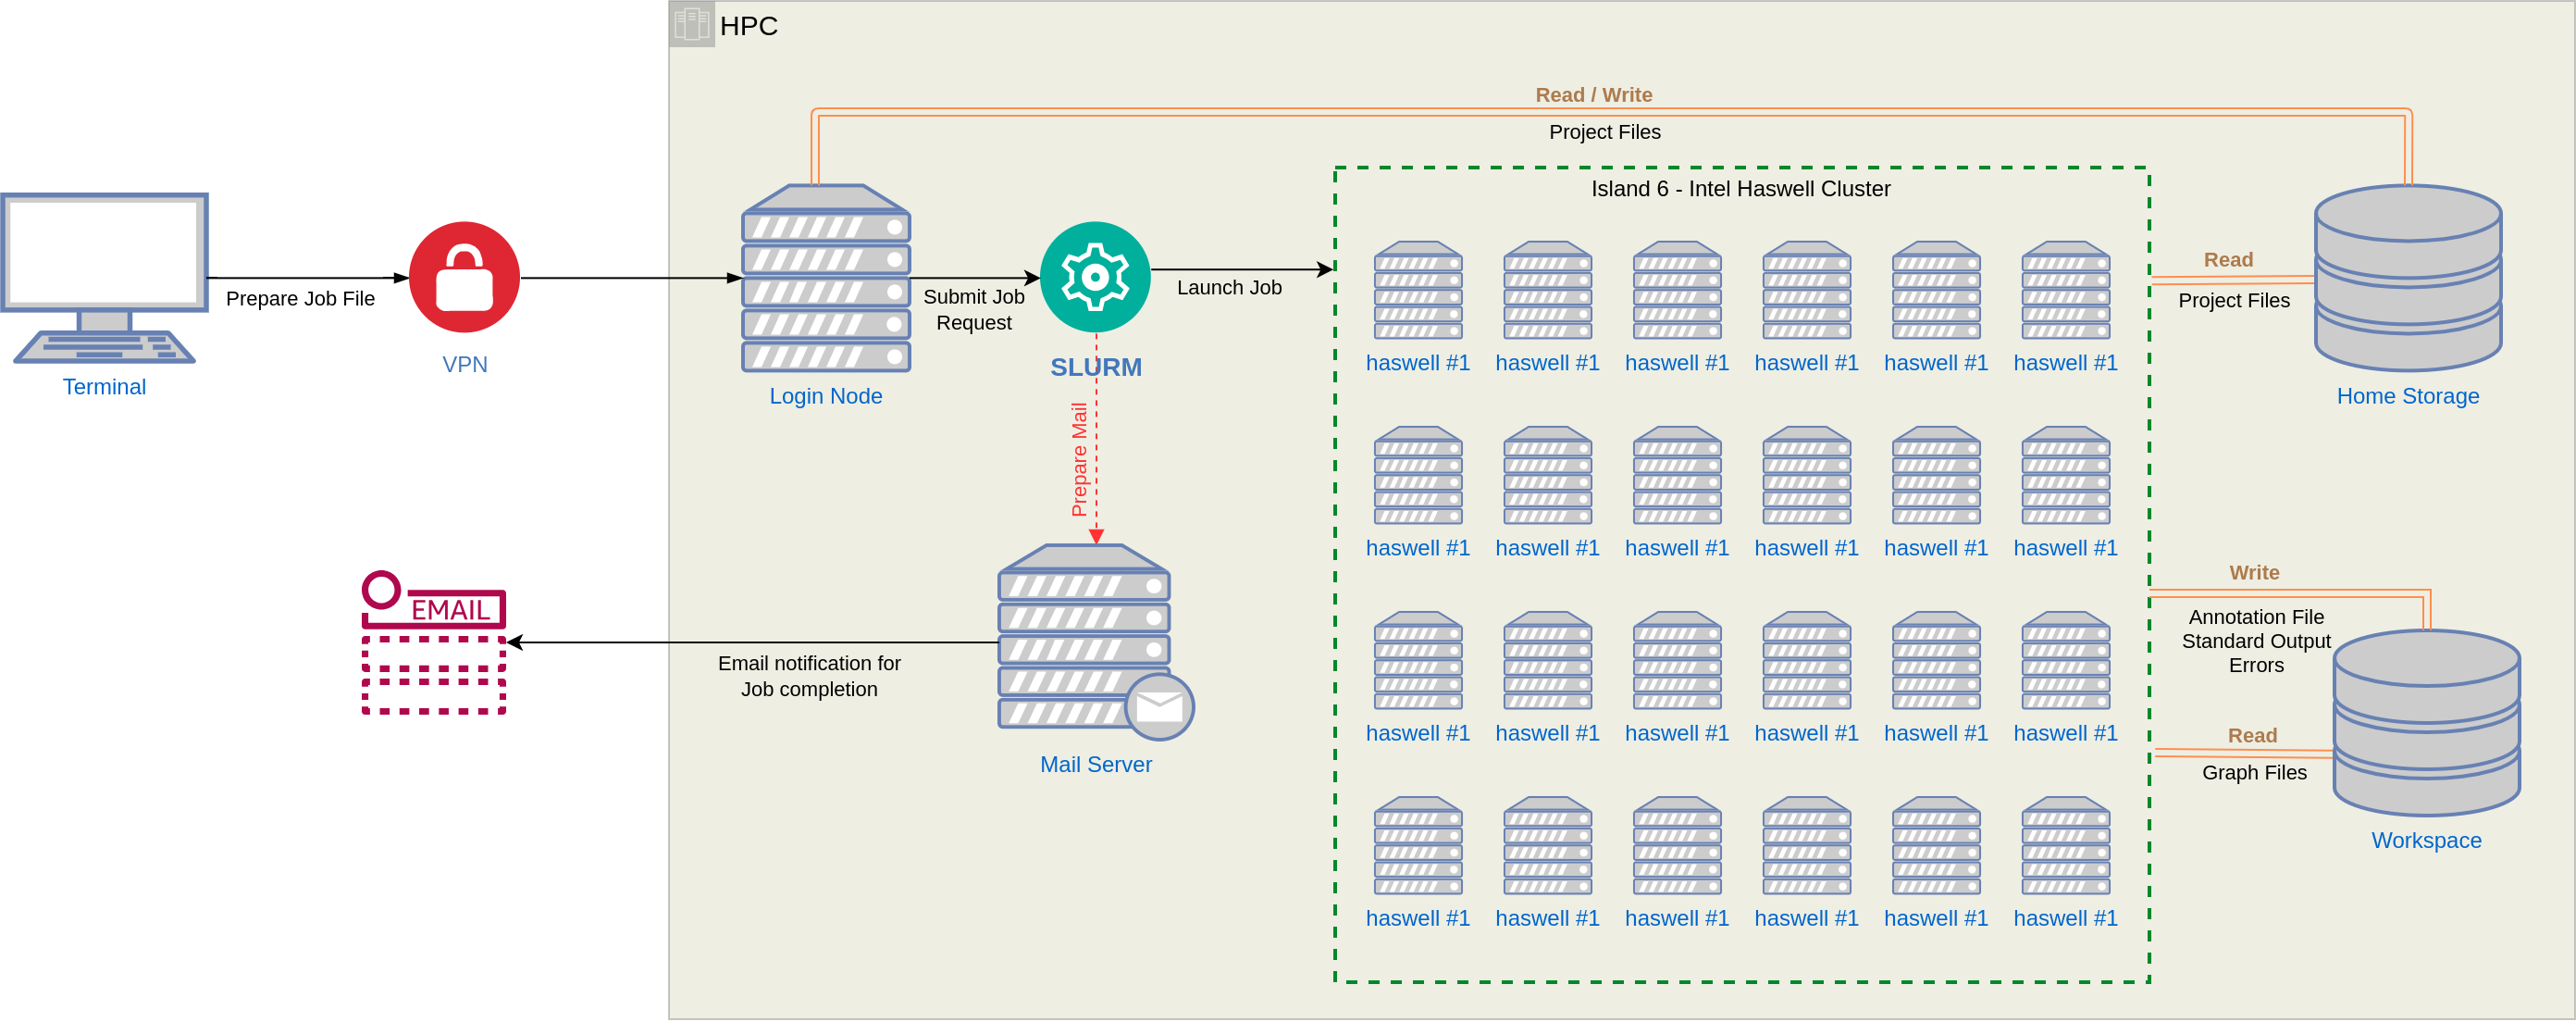
\includegraphics[width=0.95\textwidth]{Figures/DatasetAnnotation.png}
	\caption{HPC pipeline to annotate mean payoff graphs
	\label{fig:HPCAnnotation}}
\end{figure}
\FloatBarrier
The figure \ref{fig:HPCAnnotation} above highlights the pipeline used to annotate mean payoff graphs.
\newline For illustrative purposes, we omitted the following details:
\begin{itemize}
	\item The SLURM manager splits the graph files and partition them along the computing nodes.
	\item Each node produces its own annotation file, which is \textbf{unique} per computing node. So we do not have any race condition.\footnote{Processes that access the same file.} 
	\item Each of the standard output and error streams is transfered to a file, which is \textbf{unique} per computing node.
	\item Once all jobs terminate, we have a helper script that concatenate all the results into a single file.
\end{itemize} 

\begin{figure}[H]
	\centering
	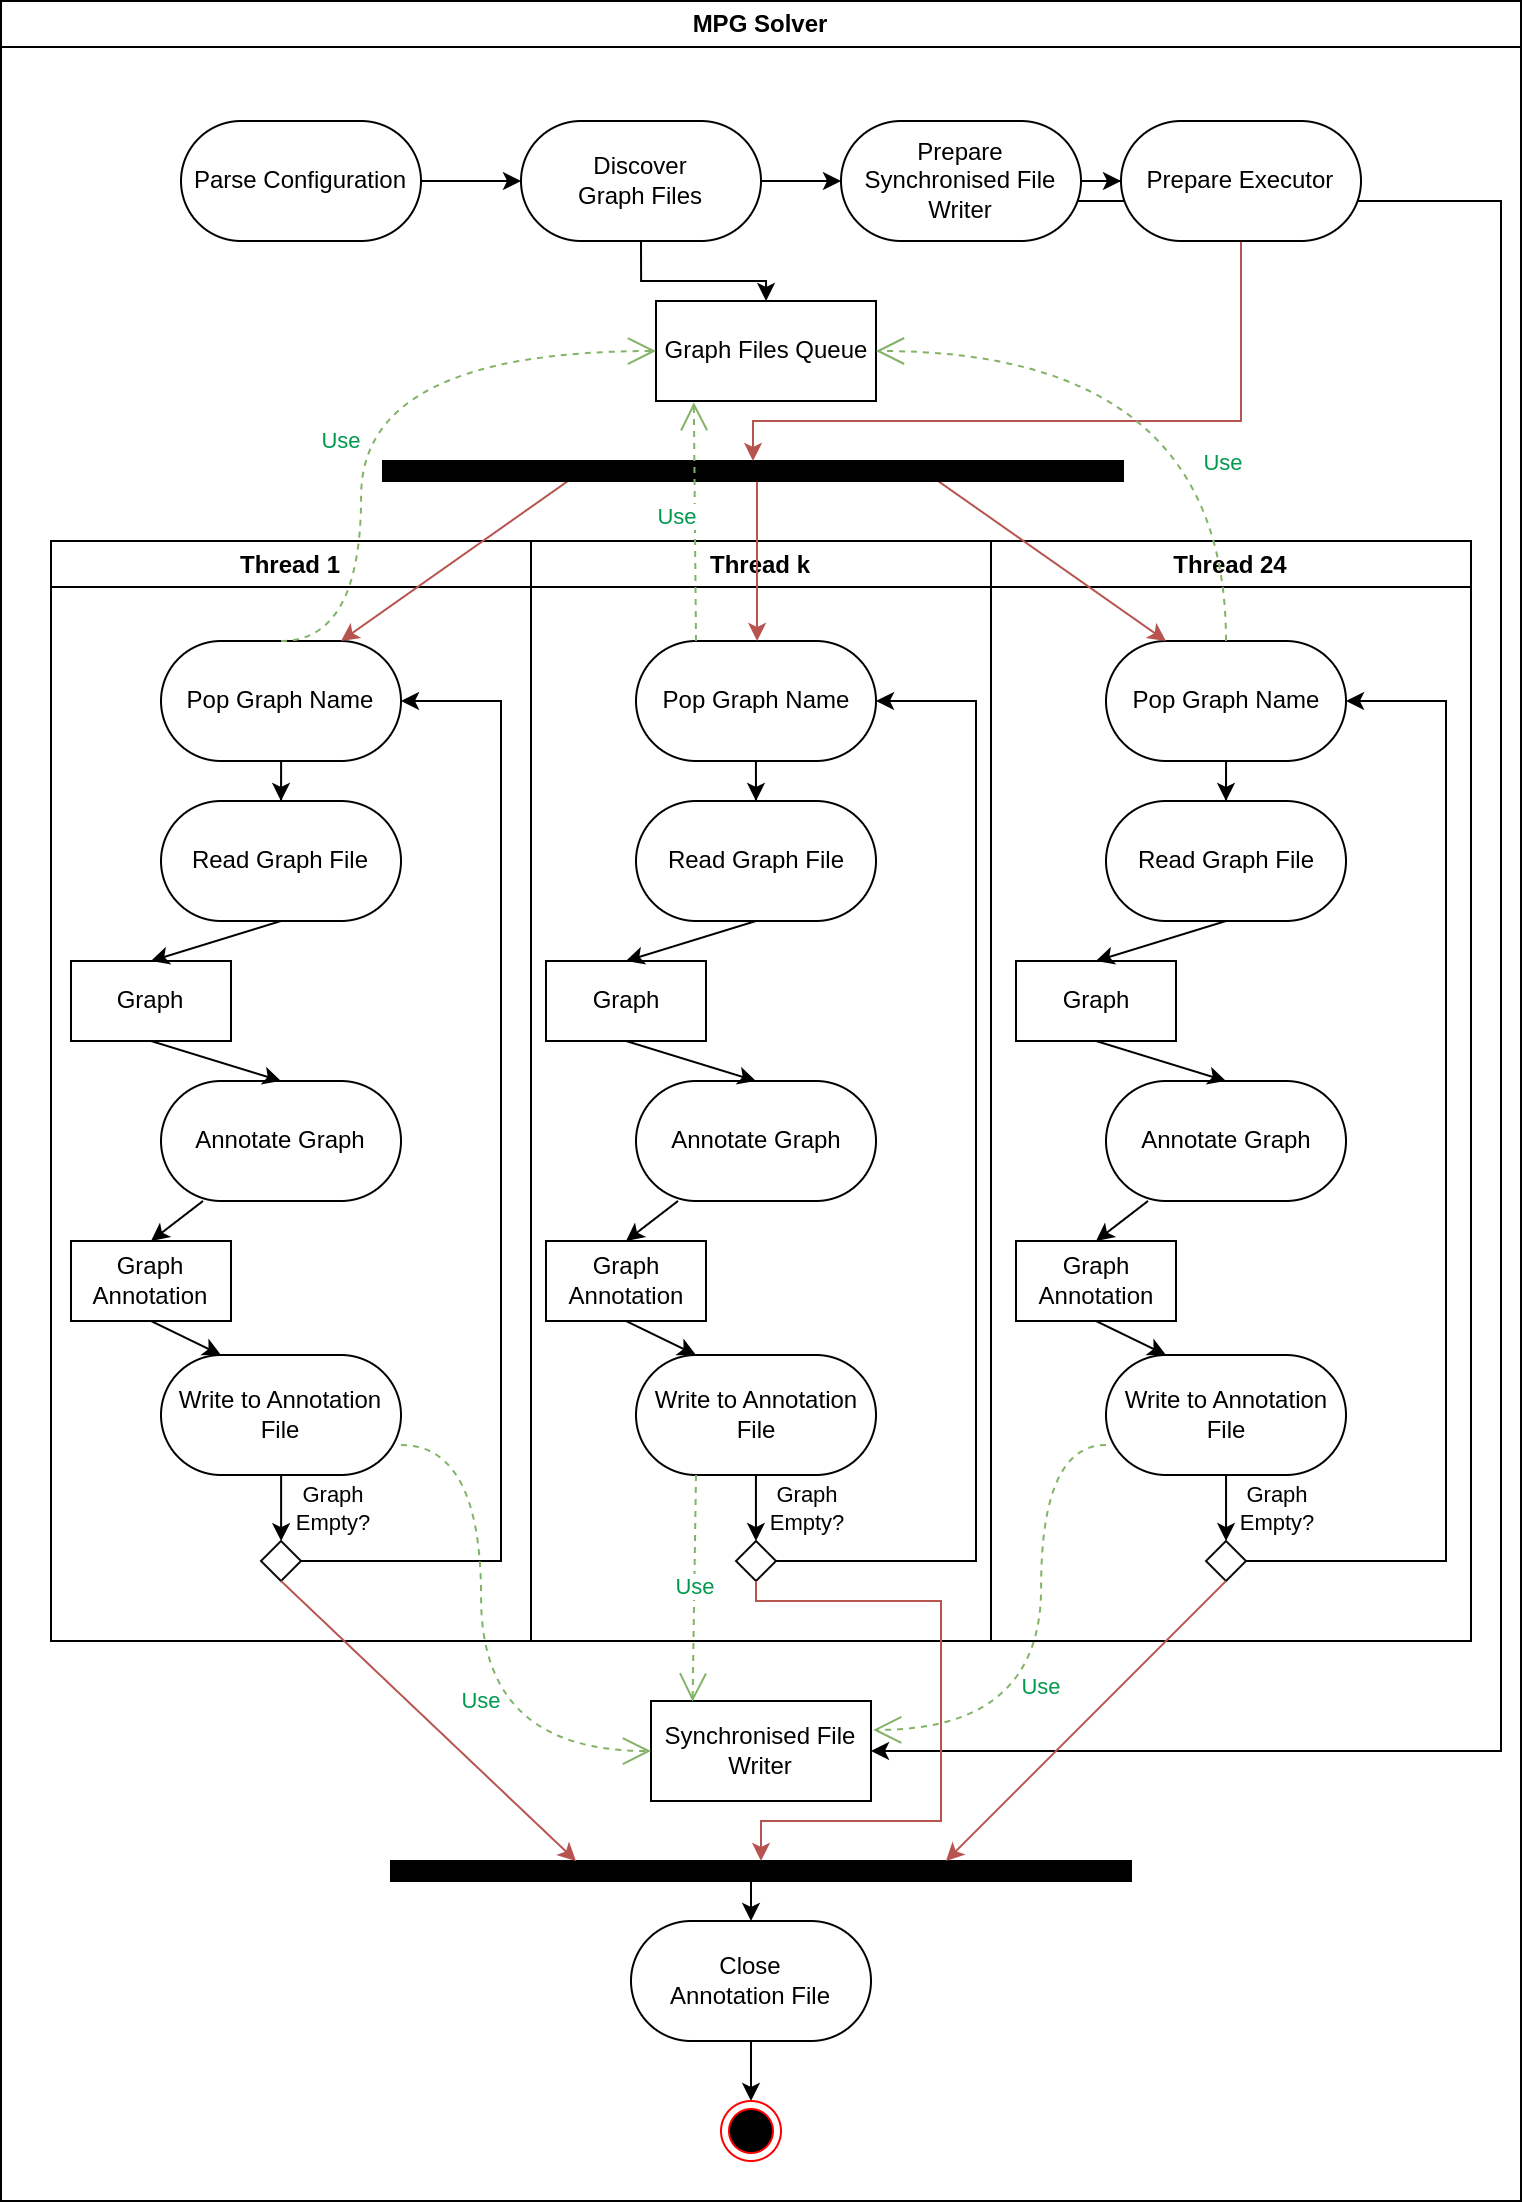
\includegraphics[width=0.85\textwidth]{Figures/AnnotationThreads.png}
	\caption{Activity diagram describing the behaviour of a node
		\label{fig:HPCAnnotationProcess}}
\end{figure}
\FloatBarrier
\newpage
\subsection{Results}
\begin{table}[h]
	\small
	\begin{tabularx}{\textwidth}{| p{1.5cm} | p{1.2cm} | p{2cm} | p{2cm} | X | X | X |}
		\hline
		
		Dataset & Size & Cardinality & Annotated & Linear Bound & Early Stopping & Time  \\
		\hline
		Dense & ? & 160000 & 160000 &\cmark &  \cmark & \\	
		\hline
		Sparse & ? & 160000& 150000  & \cmark &  \xmark & \\	
		\hline
	\end{tabularx}
	\caption{List of heuristics used by the solver
		\label{table:SolverResults}}
\end{table}
\FloatBarrier